\documentclass[a4paper, 14pt]{extarticle}
\usepackage[english,russian]{babel}
\usepackage[T1]{fontenc}
\usepackage[utf8]{inputenc}
\usepackage{fontspec}
\usepackage{indentfirst}
\usepackage{enumitem}
\usepackage{graphicx}
\usepackage[
  left=20mm,
  right=10mm,
  top=20mm,
  bottom=20mm
]{geometry}
\usepackage{parskip}
\usepackage{titlesec}
\usepackage{xurl}
\usepackage{hyperref}
\usepackage{float}
\usepackage[
  figurename=Рисунок,
  labelsep=endash,
  justification=centering
]{caption}
\usepackage[outputdir=build, newfloat]{minted}
\usepackage{chngcntr}

\selectlanguage{russian}

\hypersetup{
  colorlinks=true,
  linkcolor=black,
  filecolor=blue,
  urlcolor=blue,
}

\renewcommand*{\labelitemi}{---}
\setmainfont{Times New Roman}
\setmonofont{JetBrains Mono}[
  SizeFeatures={Size=11},
]

\newenvironment{code}{\captionsetup{type=figure}}{}
\BeforeBeginEnvironment{code}{\bigskip}
\AfterEndEnvironment{code}{\bigskip}

\setminted{
  fontsize=\footnotesize,
}

\setlength{\parskip}{6pt}

\setlength{\parindent}{1.25cm}
\setlist[itemize]{itemsep=0em,topsep=0em,parsep=0em,partopsep=0em,leftmargin=2.0cm,wide}
\setlist[enumerate]{itemsep=0em,topsep=0em,parsep=0em,partopsep=0em,leftmargin=2.0cm,wide}

\renewcommand{\thesection}{\indent\arabic{section}.}
\renewcommand{\thesubsection}{\indent\thesection\arabic{subsection}.}
\renewcommand{\thesubsubsection}{\indent\thesubsection\arabic{subsubsection}.}

\titleformat{\section}{\normalfont\bfseries}{\thesection}{0.5em}{}
\titleformat{\subsection}{\normalfont\bfseries}{\thesubsection}{0.5em}{}
\titleformat{\subsubsection}{\normalfont\bfseries}{\thesubsubsection}{0.5em}{}

\titleformat*{\section}{\normalfont\bfseries}
\titleformat*{\subsection}{\normalfont\bfseries}
\titleformat*{\subsubsection}{\normalfont\bfseries}

\titlespacing{\section}{\parindent}{\parskip}{\parskip}
\titlespacing{\subsection}{\parindent}{\parskip}{\parskip}
\titlespacing{\subsubsection}{\parindent}{\parskip}{\parskip}

\linespread{1.5}
\renewcommand{\baselinestretch}{1.5}

\begin{document}

\begin{titlepage}
  \vspace{0pt plus2fill}
  \noindent

  \vspace{0pt plus6fill}
  \begin{center}
    Санкт-Петербургский национальный исследовательский университет
    информационных технологий, механики и оптики

    \vspace{0pt plus3fill}

    Факультет инфокоммуникационных технологий

    Направление подготовки 11.03.02

    \vspace{0pt plus2fill}

    Лабораторная работа №2

    <<Основы объектно-ориентированного проектирования в Java>>

  \end{center}

  \vspace{0pt plus6fill}
  \begin{flushright}
    Выполнил: \\
    Швалов Даниил Андреевич

    Группа: К33211

    Проверил: \\
    Иванов Сергей Евгеньевич
  \end{flushright}

  \vspace{0pt plus5fill}
  \begin{center}
    Санкт-Петербург

    2024
  \end{center}
\end{titlepage}

\setcounter{page}{2}

\section*{Введение}

Цель работы:
\begin{itemize}
  \item создание приложений, реализующих различные операции над элементами
  массивов;
  \item получение навыков объектно-ориентированного анализа и проектирование
  классов для задач из различных предметных областей.
\end{itemize}

\section*{Ход работы}

\subsection*{
  Упражнение 1. Использование аргументов командной строки и разбор массива args
}

В данном упражнении необходимо создать программу, в которой программа генерирует
случайное число от 1 до 5, а пользователь пытается угадать это число. На рисунке
\ref{fig:task-1-1} показан исходный код получившейся программы. На рисунке
\ref{fig:task-1-2} приведен пример работы программы.

\begin{figure}[H]
  \centering
  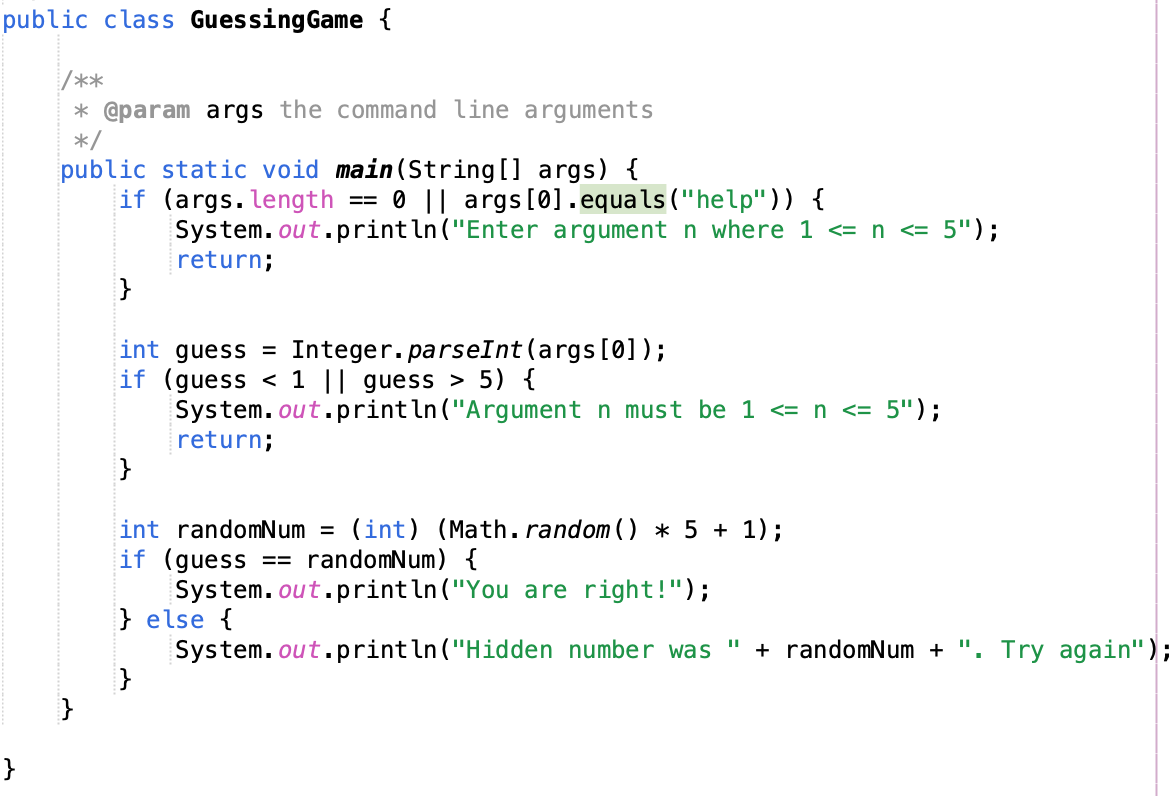
\includegraphics[width=0.9\textwidth]{images/task-1/1.png}
  \caption{Исходный код программы}
  \label{fig:task-1-1}
\end{figure}

\begin{figure}[H]
  \centering
  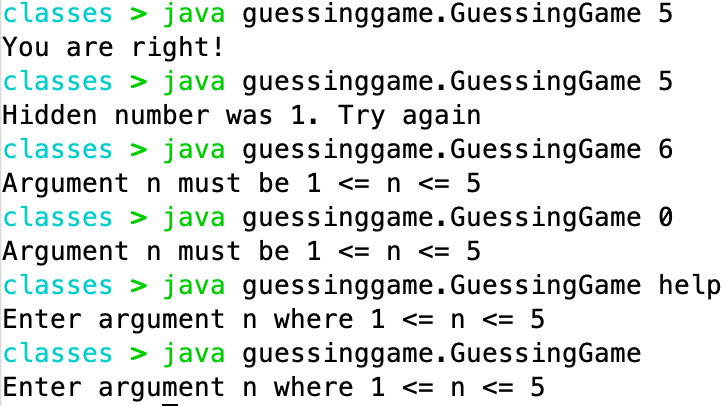
\includegraphics[width=0.4\textwidth]{images/task-1/2.png}
  \caption{Вывод программы}
  \label{fig:task-1-2}
\end{figure}

\subsection*{
  Упражнение 2. Создание пользовательского класса и включение комментариев в код
}

В данном упражнении необходимо спроектировать классы банковской системы. На
рисунке \ref{fig:task-2-1} приведен исходный код класса
<<\foreignlanguage{english}{Account}>>. Он представляет собой информацию об
аккаунте и содержит информацию о клиенте. Для тестирования методов класса был
написан код, показанный на рисунке \ref{fig:task-2-2}. Вывод данной программы
изображен на рисунке \ref{fig:task-2-3}.

\begin{figure}[H]
  \centering
  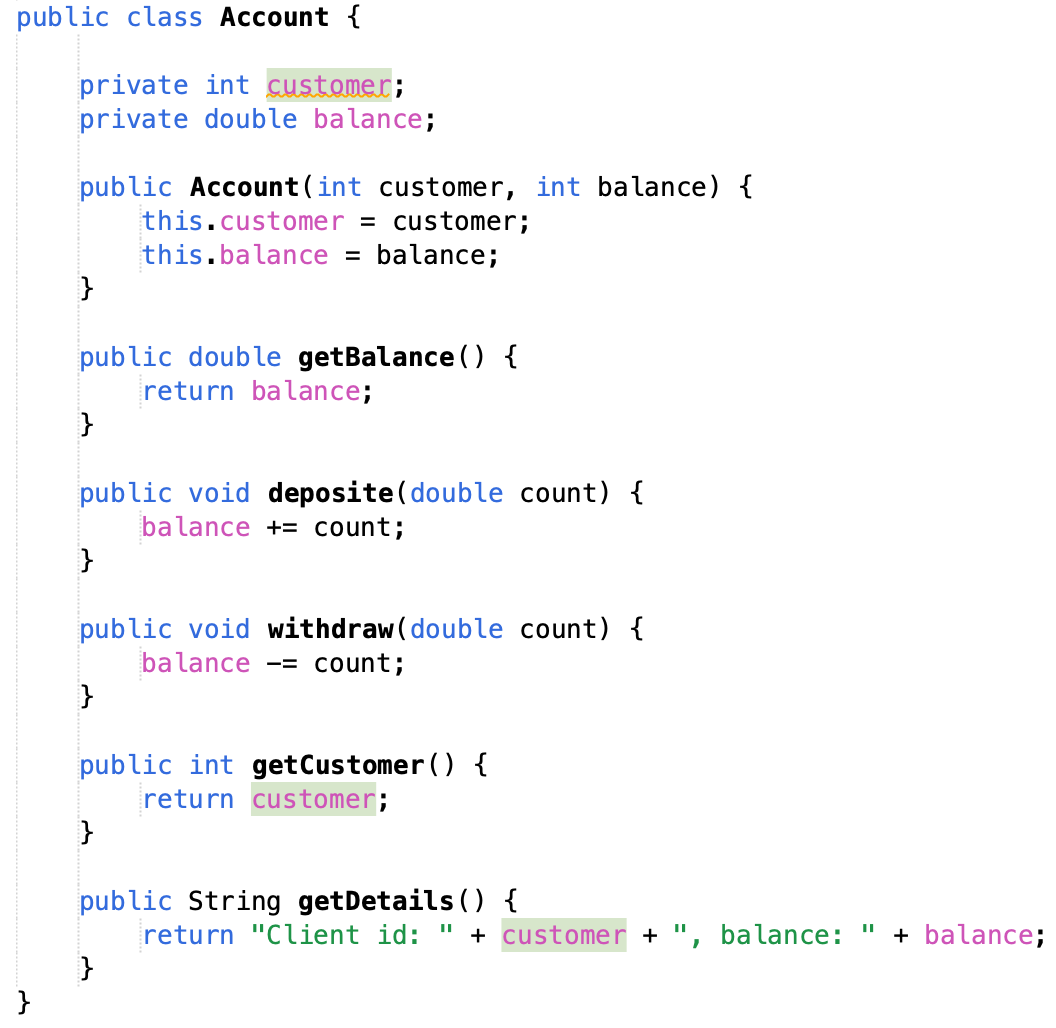
\includegraphics[width=0.6\textwidth]{images/task-2/1.png}
  \caption{Исходный код класса <<\foreignlanguage{english}{Account}>>}
  \label{fig:task-2-1}
\end{figure}

\begin{figure}[H]
  \centering
  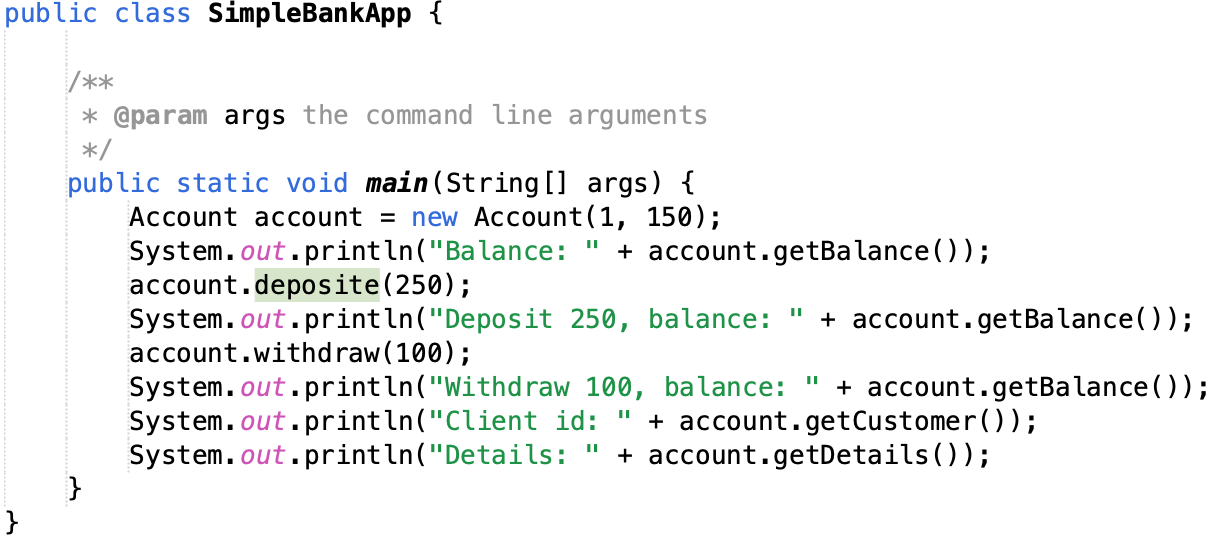
\includegraphics[width=0.9\textwidth]{images/task-2/2.png}
  \caption{Код для тестирования класса <<\foreignlanguage{english}{Account}>>}
  \label{fig:task-2-2}
\end{figure}

\begin{figure}[H]
  \centering
  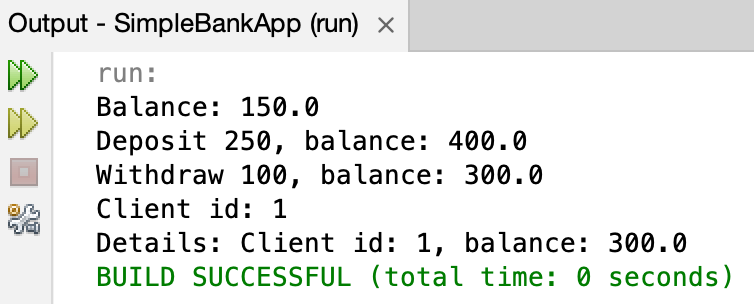
\includegraphics[width=0.6\textwidth]{images/task-2/3.png}
  \caption{Вывод программы}
  \label{fig:task-2-3}
\end{figure}

Затем был добавлен класс <<\foreignlanguage{english}{ATM}>>, представляющий
банкомат. Он содержит метод для вывода информации о счете клиента. Исходный код
класса <<\foreignlanguage{english}{ATM}>> приведен на рисунке
\ref{fig:task-2-4}. С помощью кода, показанного на рисунке \ref{fig:task-2-5},
класс <<\foreignlanguage{english}{ATM}>> был протестирован. Вывод программы
приведен на рисунке \ref{fig:task-2-6}.

\begin{figure}[H]
  \centering
  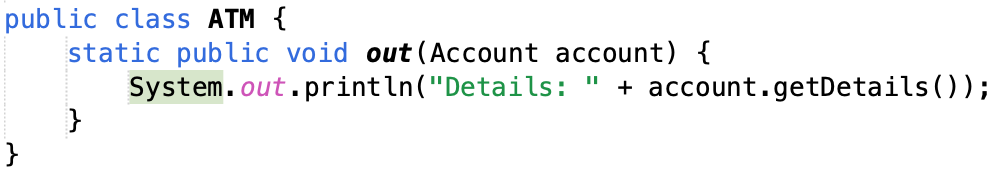
\includegraphics[width=0.8\textwidth]{images/task-2/4.png}
  \caption{Исходный код класса <<\foreignlanguage{english}{ATM}>>}
  \label{fig:task-2-4}
\end{figure}

\begin{figure}[H]
  \centering
  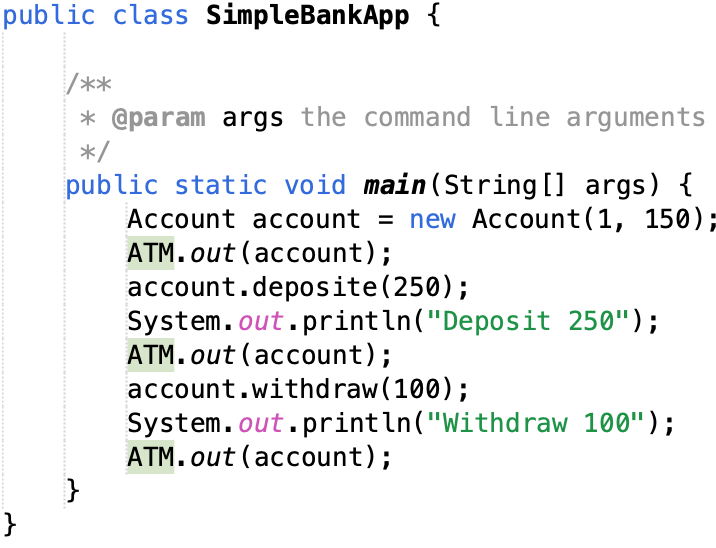
\includegraphics[width=0.7\textwidth]{images/task-2/5.png}
  \caption{Кол для тестирования класса <<\foreignlanguage{english}{ATM}>>}
  \label{fig:task-2-5}
\end{figure}

\begin{figure}[H]
  \centering
  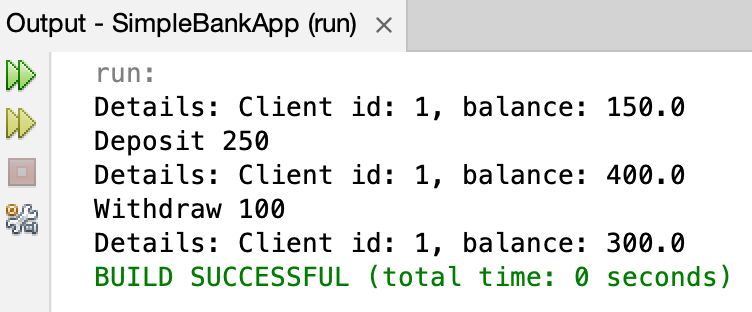
\includegraphics[width=0.5\textwidth]{images/task-2/6.png}
  \caption{Вывод программы}
  \label{fig:task-2-6}
\end{figure}

После этого в класс <<\foreignlanguage{english}{Account}>> были добавлены
документирующие комментарии. К каждому методу было добавлено описание, что
делает данный метод. Для тех методов, у которых есть параметры или возвращаемое
значение, были дописаны дополнительные комментарии. На рисунке
\ref{fig:task-2-7} приведен получившийся исходный код с комментариями.

\begin{figure}[H]
  \centering
  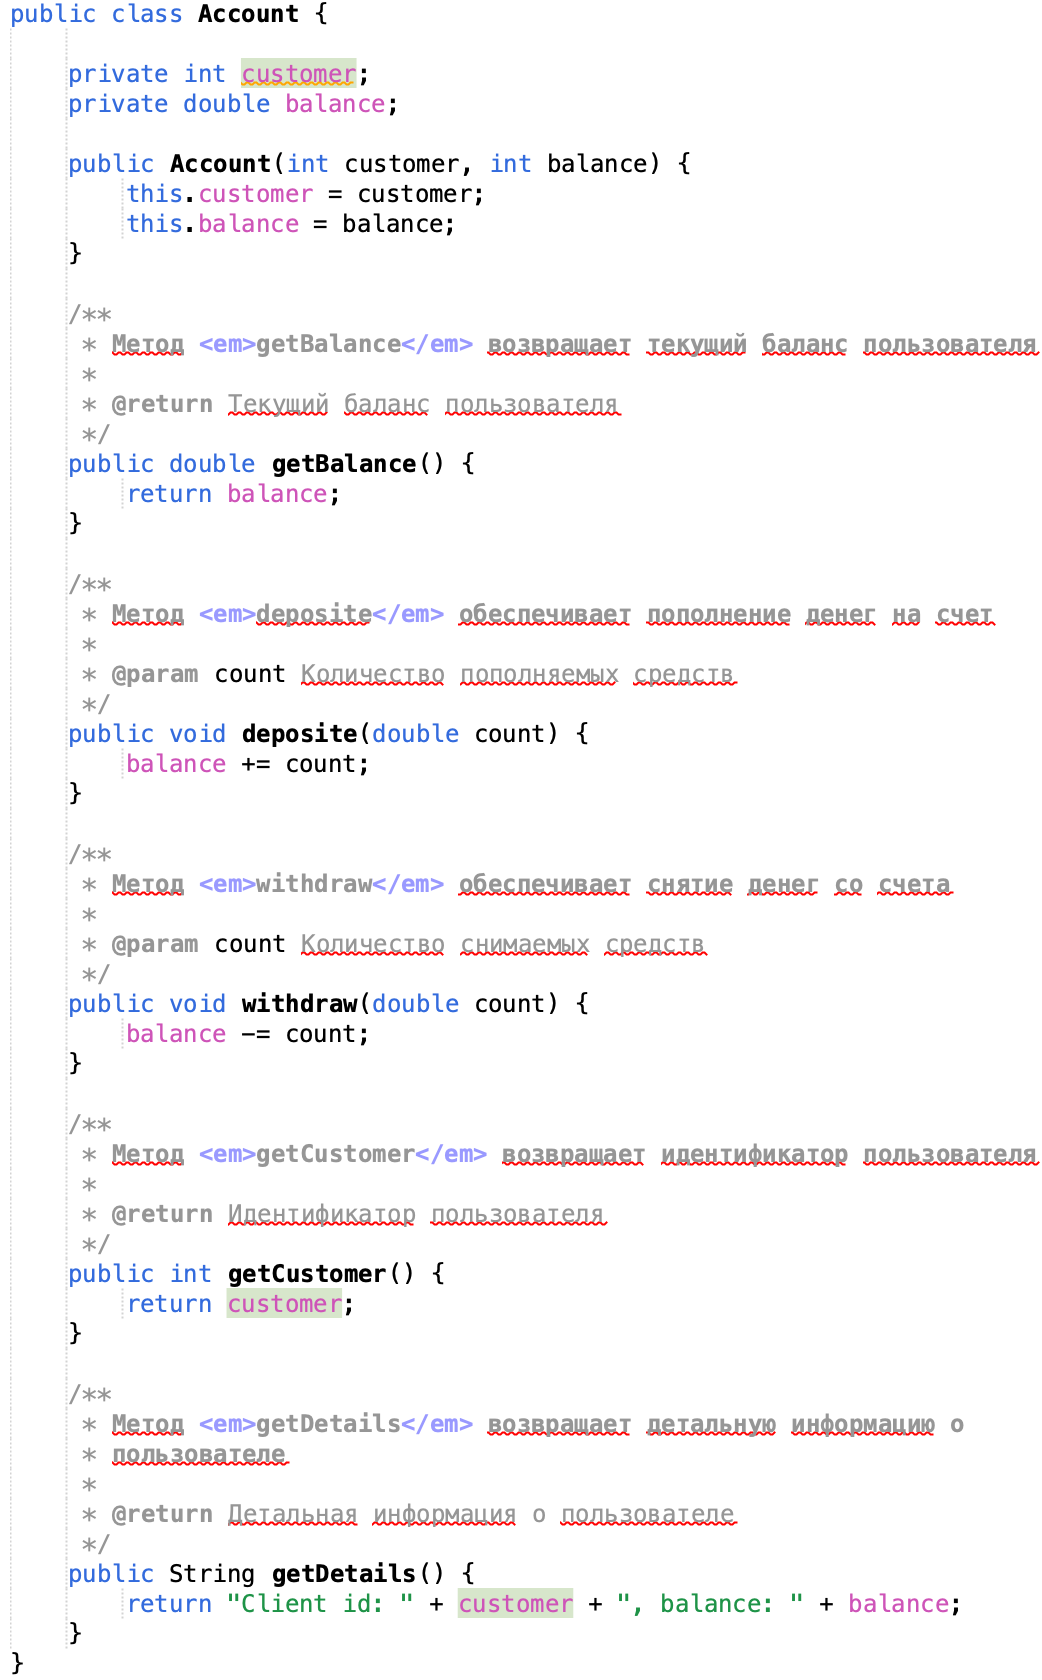
\includegraphics[width=0.7\textwidth]{images/task-2/7.png}
  \caption{Исходный код класса <<\foreignlanguage{english}{Account}>>}
  \label{fig:task-2-7}
\end{figure}

Затем был настроен javadoc, чтобы в сгенерированную документацию добавлялись
авторы и версии. Для этого в параметры javadoc были добавлены флаги <<-author>>
и <<-version>> (рисунок \ref{fig:task-2-8}). После генерации документации была
создана страница, показанная на рисунке \ref{fig:task-2-9}. Как видно, на ней
отображена та информация, которая была добавлена в комментарии.

\begin{figure}[H]
  \centering
  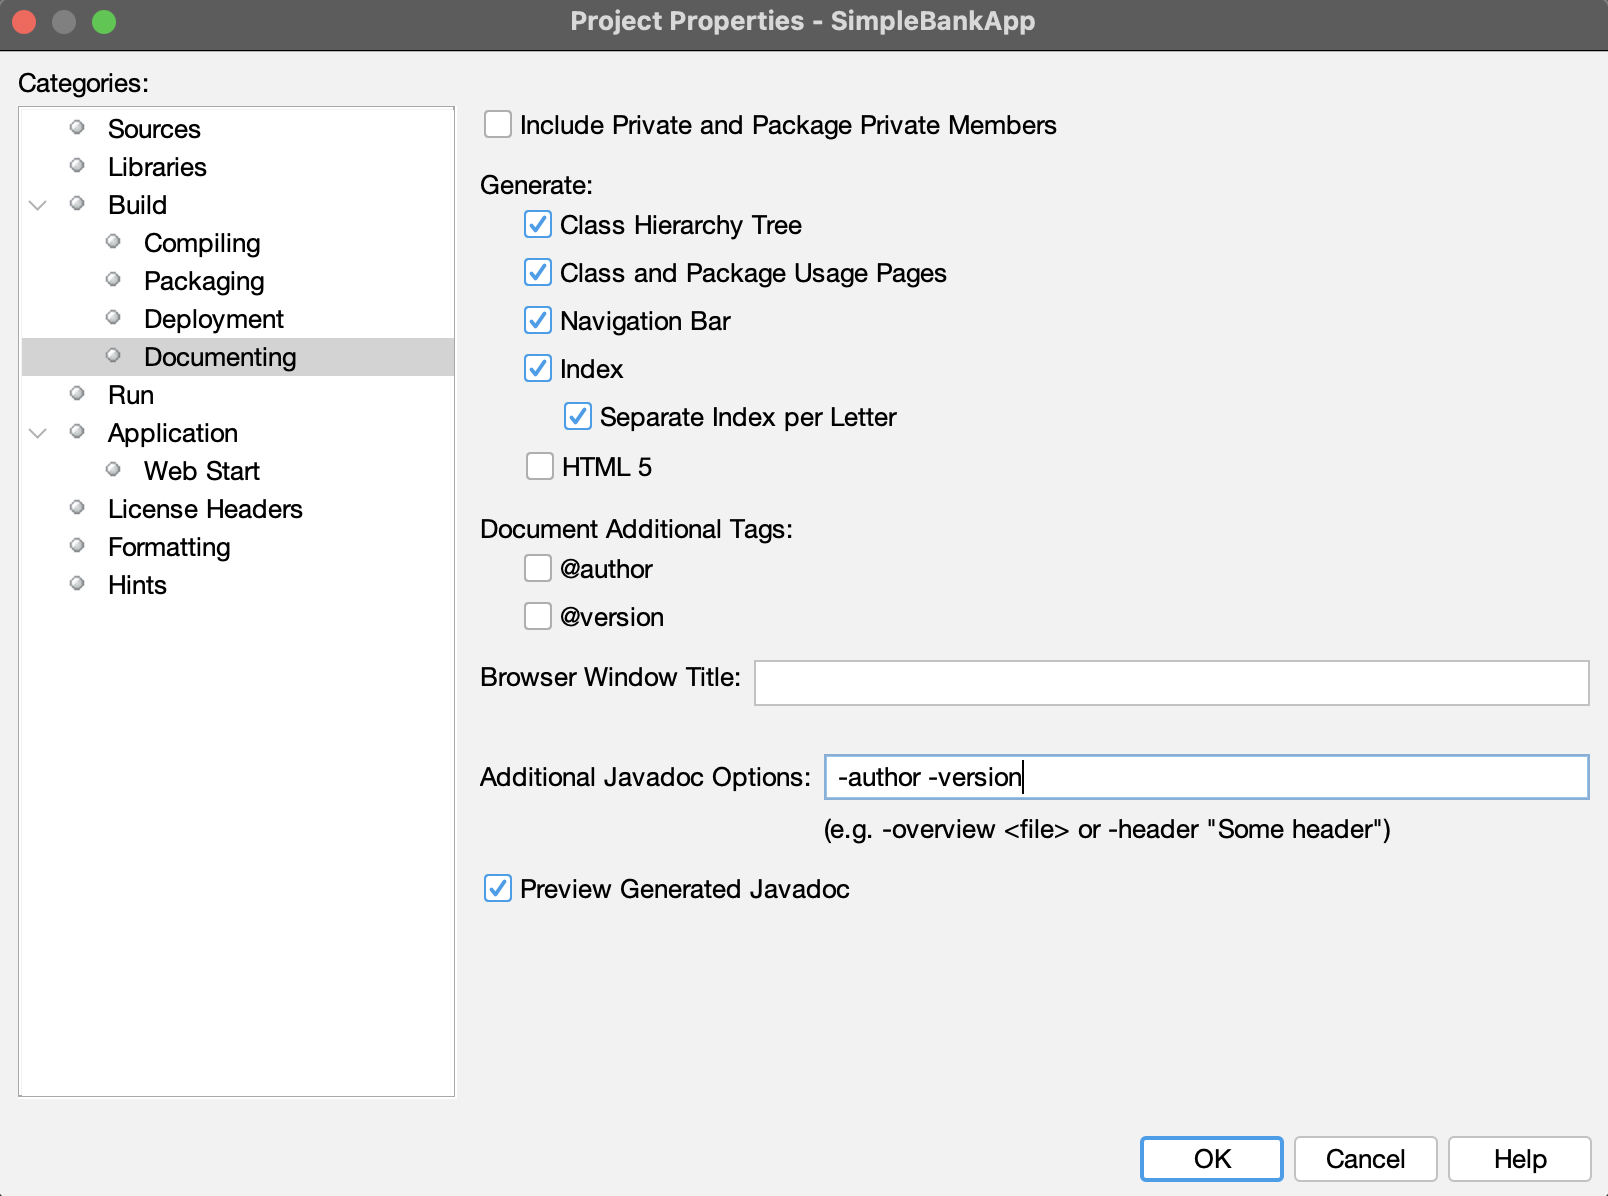
\includegraphics[width=\textwidth]{images/task-2/8.png}
  \caption{Настройка javadoc}
  \label{fig:task-2-8}
\end{figure}

\begin{figure}[H]
  \centering
  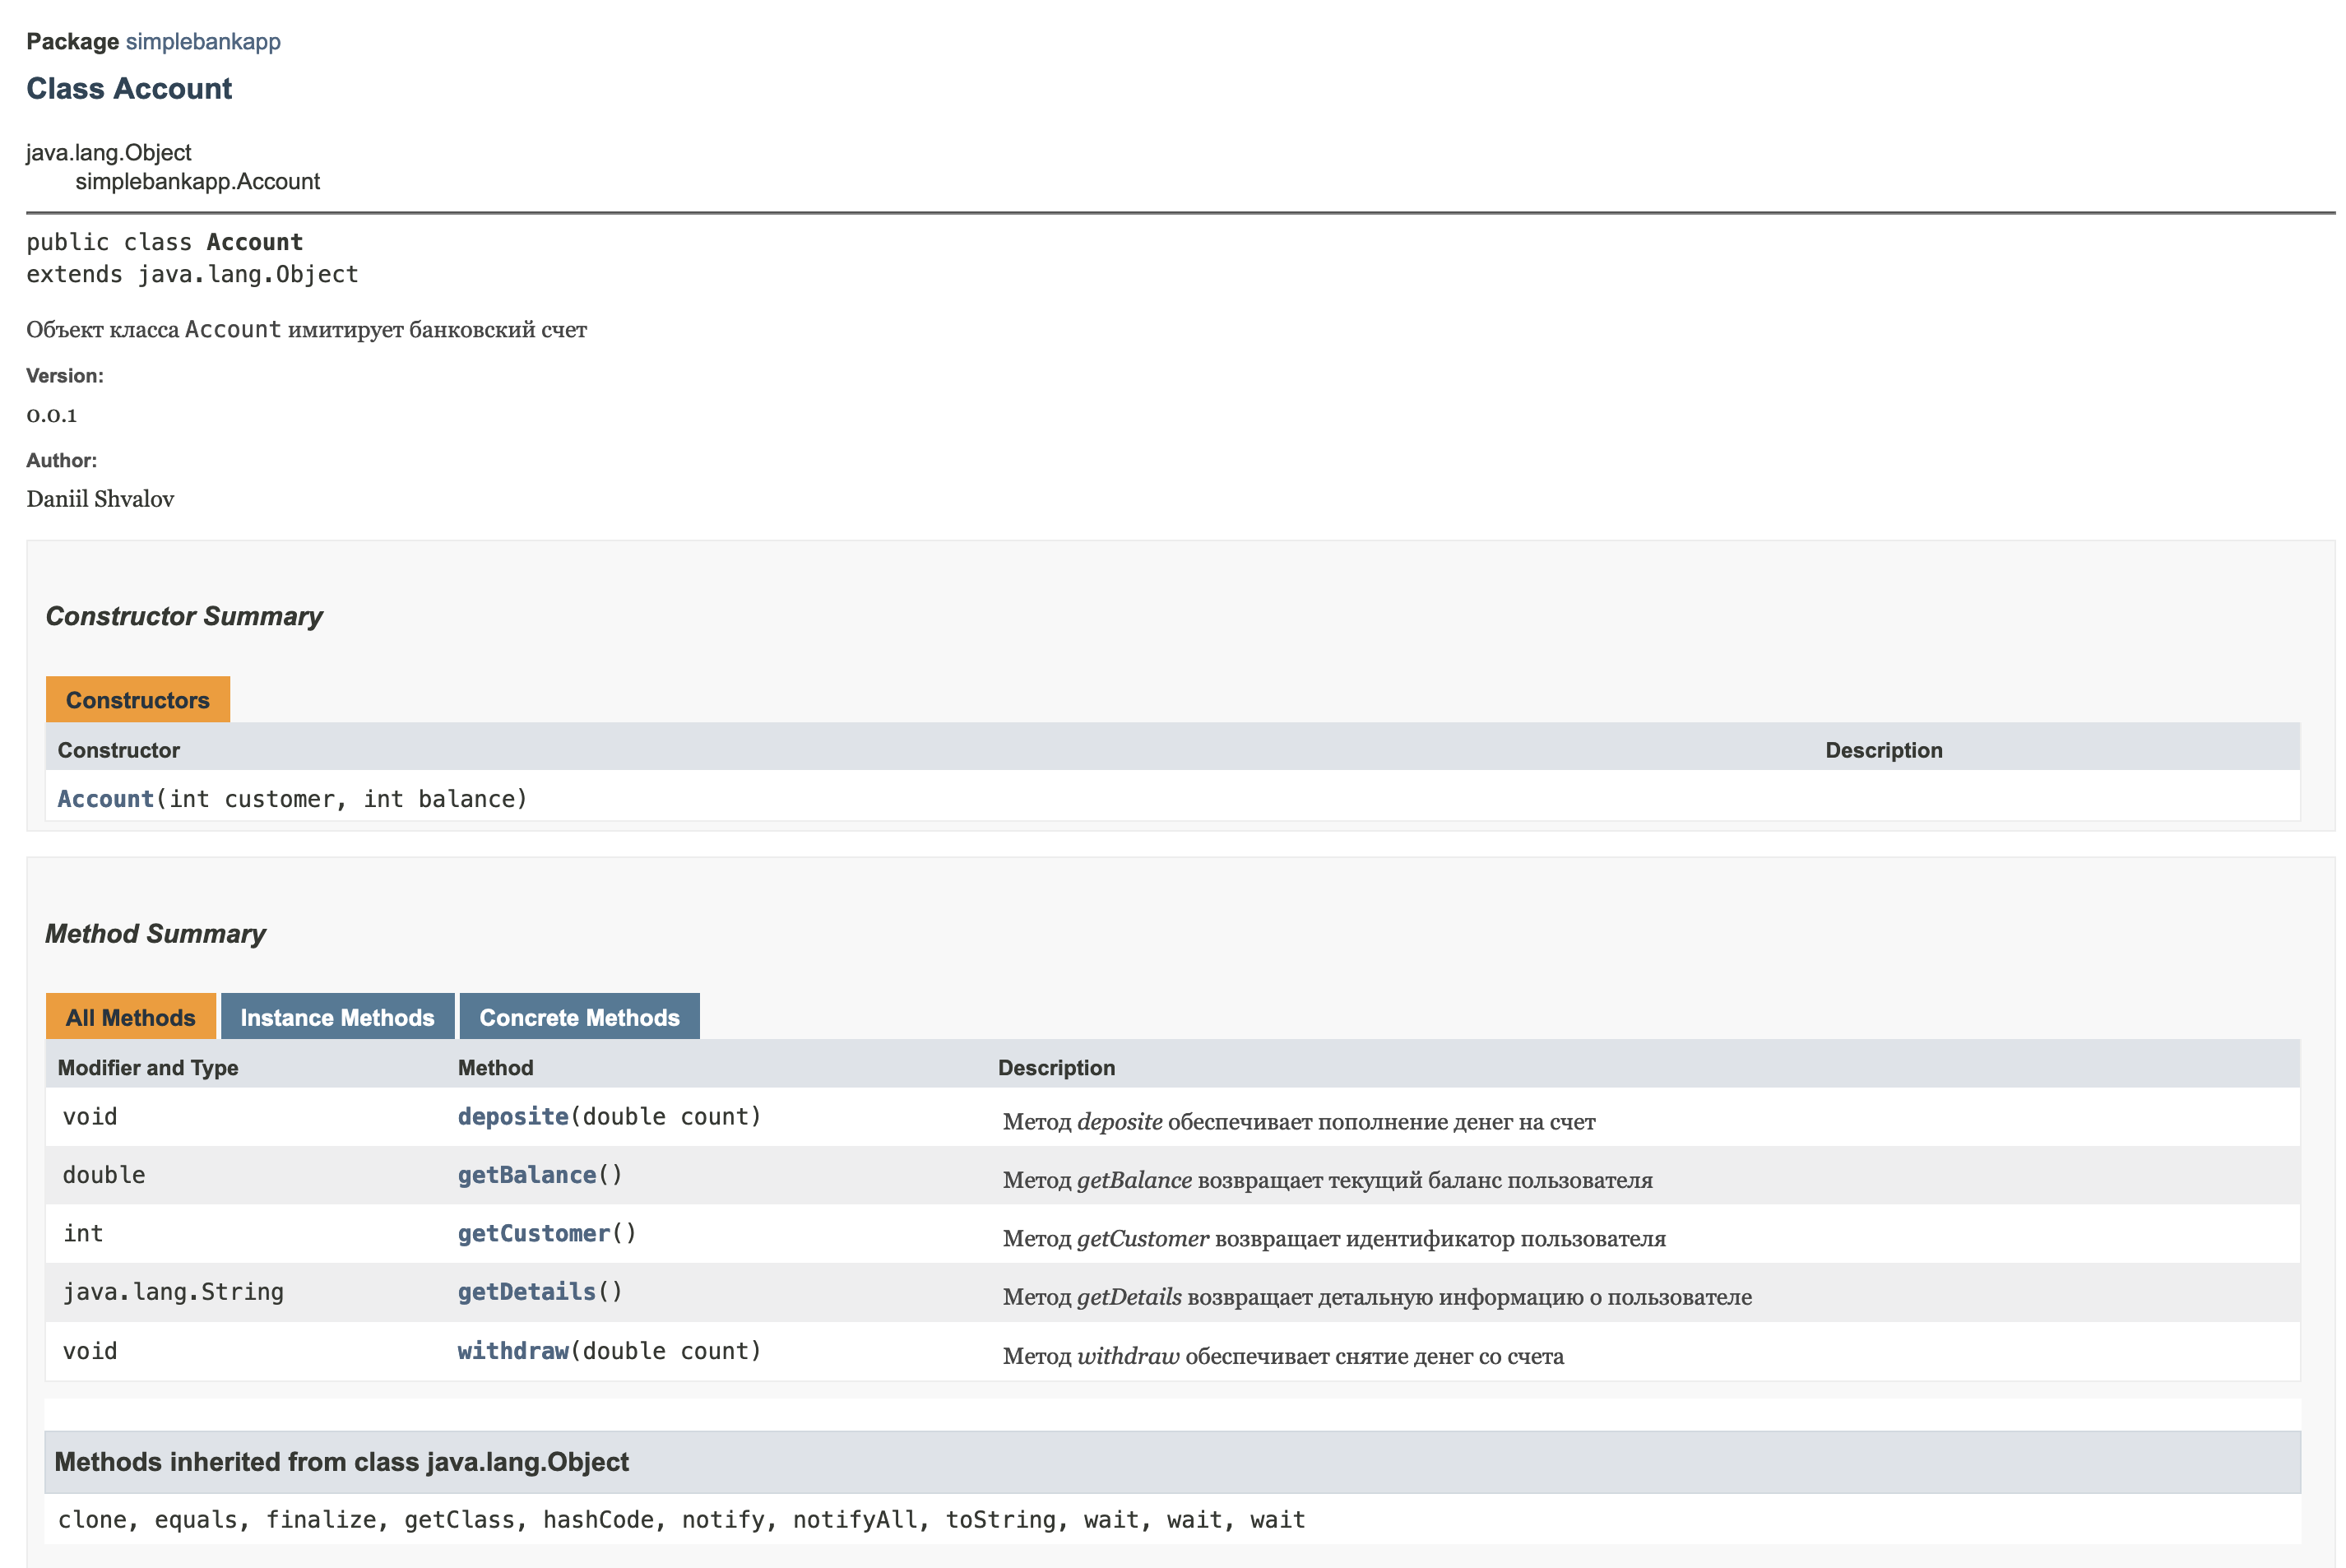
\includegraphics[width=\textwidth]{images/task-2/9.png}
  \caption{Сгенерированная документация}
  \label{fig:task-2-9}
\end{figure}

\subsection*{
  Упражнение 3. Отладка приложений в интегрированной среде разработки.
}

В данном упражнении необходимо научиться использовать отладчик. Для этого был
создан класс <<\foreignlanguage{english}{Shirt}>>, при создании которого поля
класса заполняются некоторым значениями по умолчанию. Также в данный класс был
добавлен метод для вывода информации о классе. Исходный код класса приведен на
рисунке \ref{fig:task-3-1}.

После этого был создан класс <<\foreignlanguage{english}{ShirtTest}>>, который
тестирует работу класса <<\foreignlanguage{english}{Shirt}>>. Исходный код
данного класса приведен на рисунке \ref{fig:task-3-2}.

\begin{figure}[H]
  \centering
  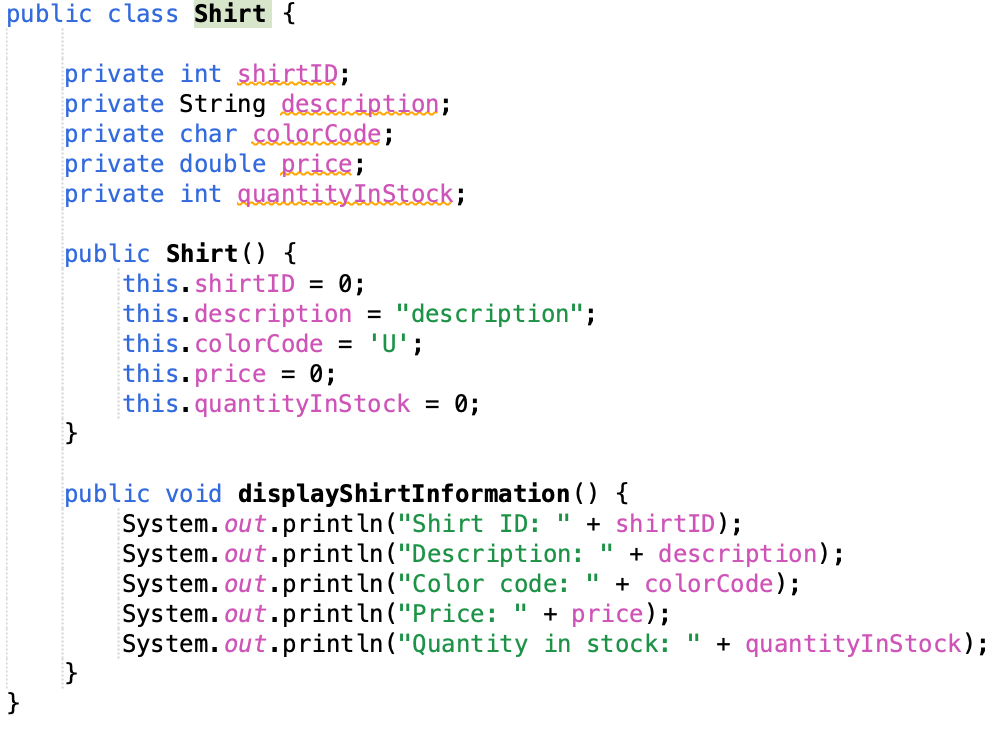
\includegraphics[width=0.8\textwidth]{images/task-3/1.png}
  \caption{Исходный код класса <<\foreignlanguage{english}{Shirt}>>}
  \label{fig:task-3-1}
\end{figure}

\begin{figure}[H]
  \centering
  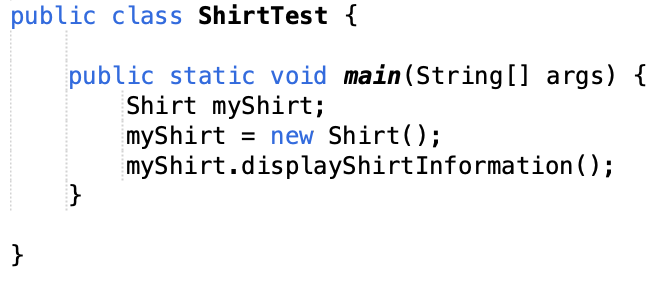
\includegraphics[width=0.6\textwidth]{images/task-3/2.png}
  \caption{Исходный код класса <<\foreignlanguage{english}{ShirtTest}>>}
  \label{fig:task-3-2}
\end{figure}

Для тестирования работы программы на 15 строке была добавлена точка останова
(рисунок \ref{fig:task-3-3}). С помощью кнопки <<\foreignlanguage{english}{Debug
  Project}>> (рисунок \ref{fig:task-3-4}) была запущена отладка программы. После
этого на экране появилась панель с информацией о значении переменных программы
(рисунок \ref{fig:task-3-5}).

\begin{figure}[H]
  \centering
  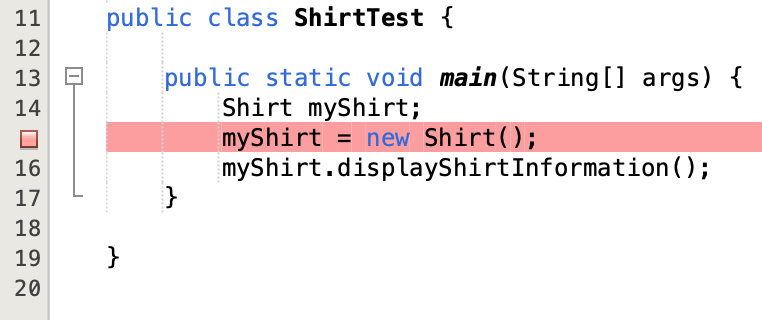
\includegraphics[width=0.7\textwidth]{images/task-3/3.png}
  \caption{Точка останова}
  \label{fig:task-3-3}
\end{figure}

\begin{figure}[H]
  \centering
  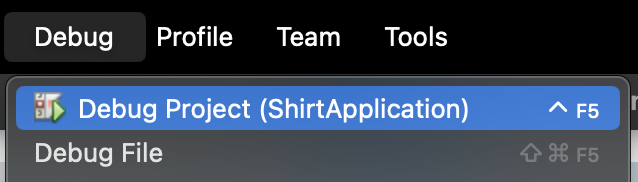
\includegraphics[width=0.6\textwidth]{images/task-3/4.png}
  \caption{Кнопка для запуска отладки программы}
  \label{fig:task-3-4}
\end{figure}

\begin{figure}[H]
  \centering
  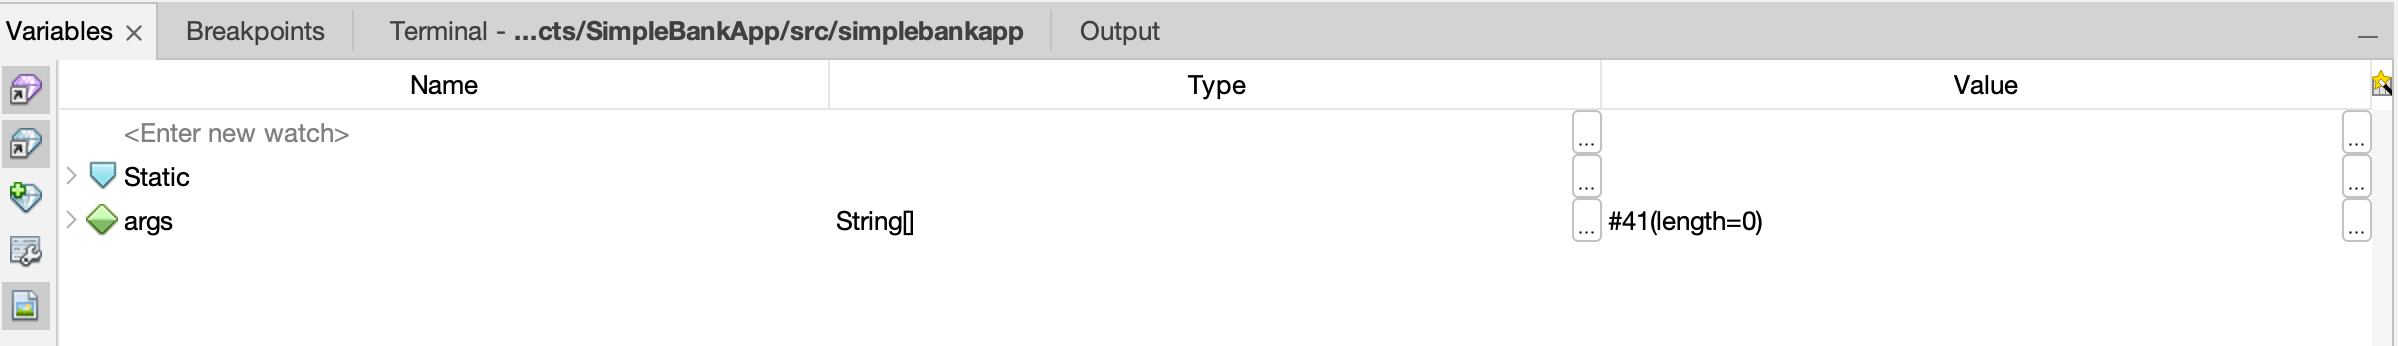
\includegraphics[width=\textwidth]{images/task-3/5.png}
  \caption{Информация о переменных}
  \label{fig:task-3-5}
\end{figure}

После нажатия на кнопку <<\foreignlanguage{english}{Step Over}>>, на панели
появились переменные класса <<\foreignlanguage{english}{Shirt}>> (рисунок
\ref{fig:task-3-6}). Затем, после нажатия на кнопку
<<\foreignlanguage{english}{Step Into}>>, на панели появились переменные метода
<<\foreignlanguage{english}{displayShirtInformation}>> (рисунок
\ref{fig:task-3-7}). Данные переменные были изменены так, как показано на
рисунке \ref{fig:task-3-8}. После продолжения выполнения программы, как видно на
рисунке \ref{fig:task-3-9}, были выведены те значения переменных, которые были
указаны в отладчике, а не те, которые были изначально.

\begin{figure}[H]
  \centering
  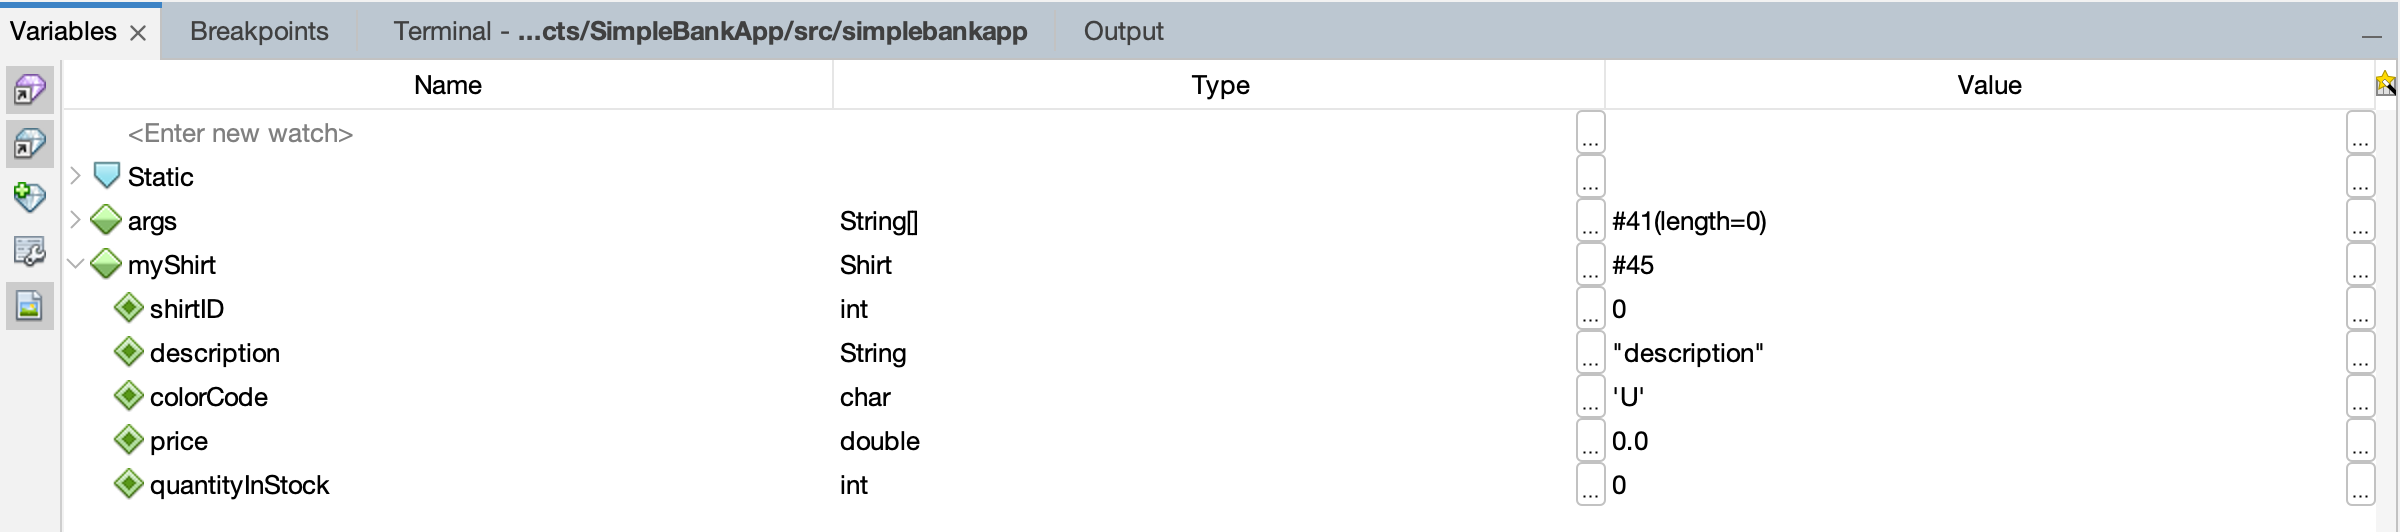
\includegraphics[width=\textwidth]{images/task-3/6.png}
  \caption{Переменные класса <<\foreignlanguage{english}{Shirt}>>}
  \label{fig:task-3-6}
\end{figure}

\begin{figure}[H]
  \centering
  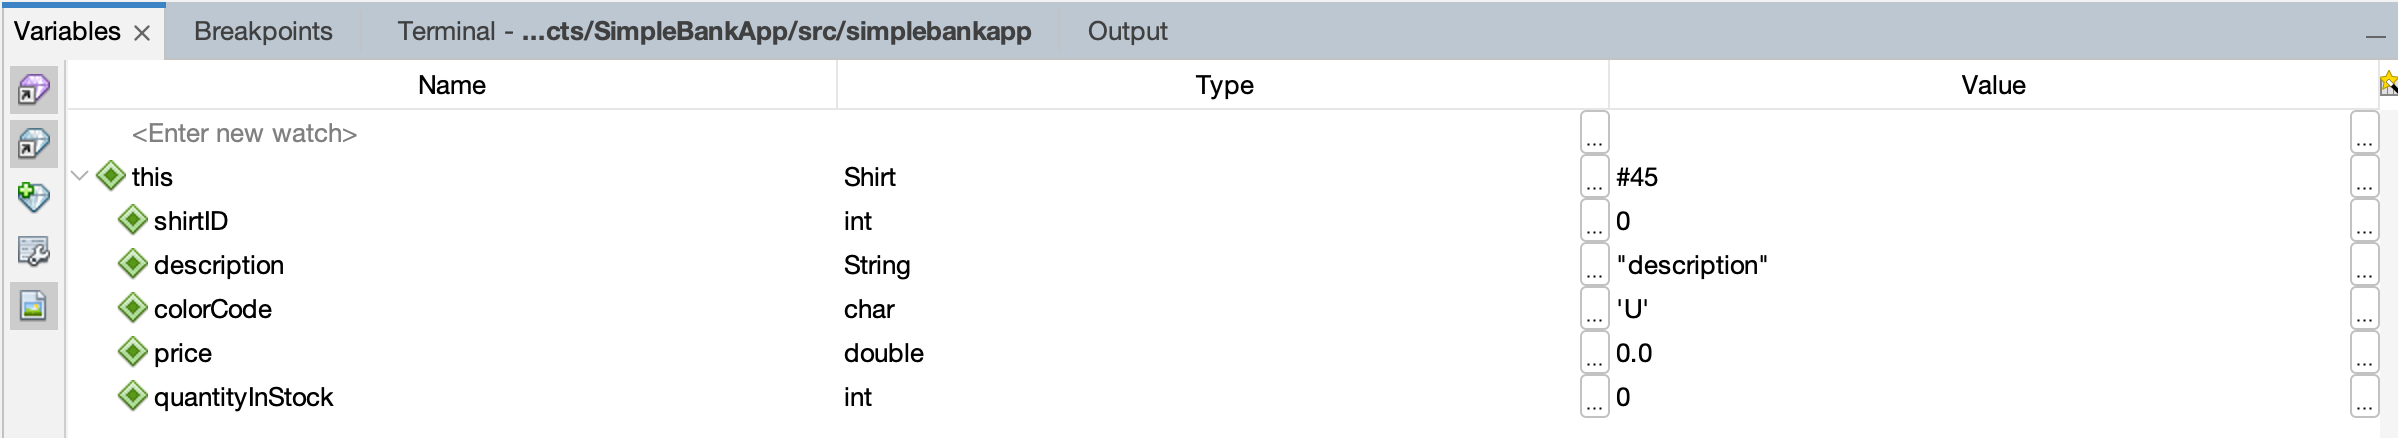
\includegraphics[width=\textwidth]{images/task-3/7.png}
  \caption{
    Переменные метода <<\foreignlanguage{english}{displayShirtInformation}>>
  }
  \label{fig:task-3-7}
\end{figure}

\begin{figure}[H]
  \centering
  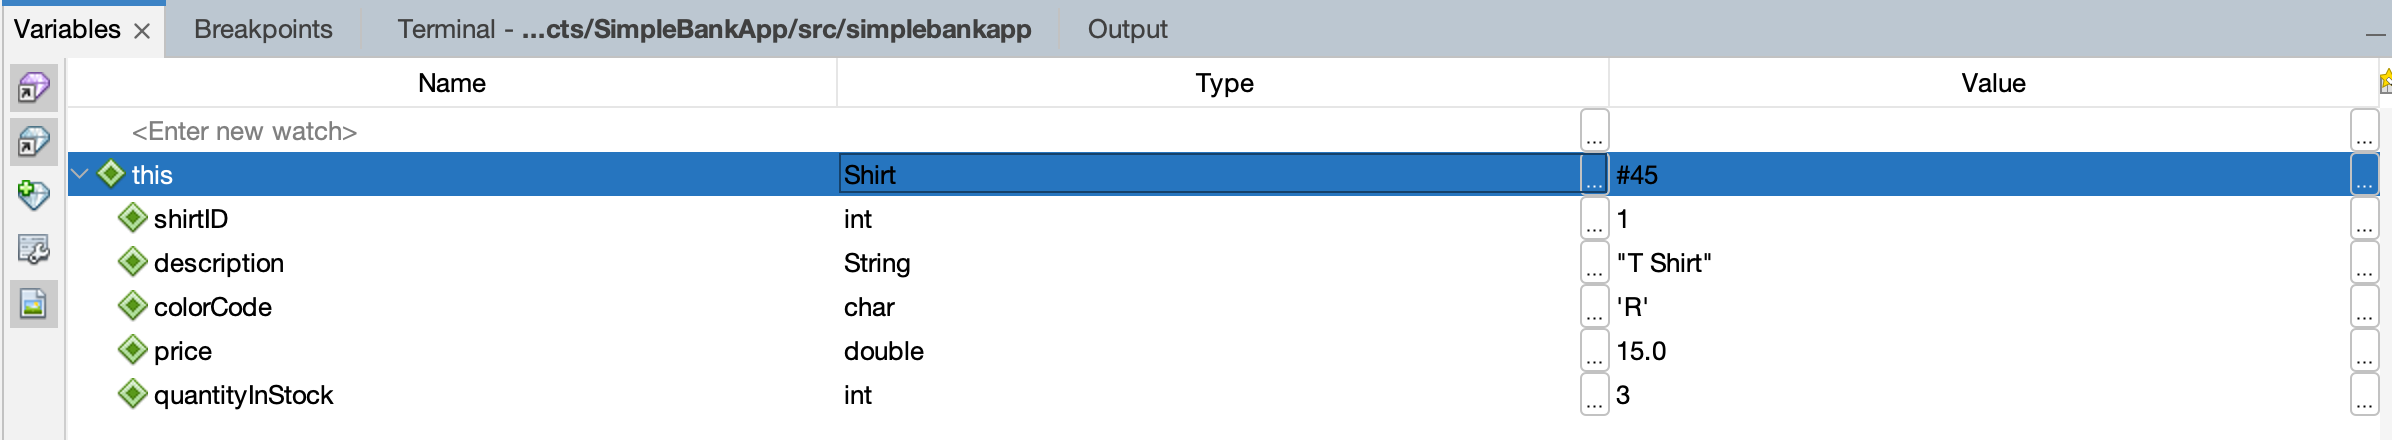
\includegraphics[width=\textwidth]{images/task-3/8.png}
  \caption{
    Измененные переменные метода
    <<\foreignlanguage{english}{displayShirtInformation}>>
  }
  \label{fig:task-3-8}
\end{figure}

\begin{figure}[H]
  \centering
  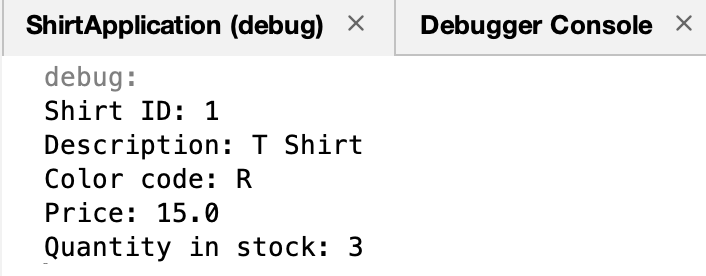
\includegraphics[width=0.6\textwidth]{images/task-3/9.png}
  \caption{Вывод программы}
  \label{fig:task-3-9}
\end{figure}

\newpage

\section*{Заключение}

В данной лабораторной работе была создана программа с использованием аргументов
командной строки. Также были созданы несколько приложений с использованием
объектно-ориентированного программирования.

Цель, поставленная в начале работы, достигнута, задачи выполнены.

\end{document}
